\documentclass[a4paper,12pt,UTF8,openright]{book}

\usepackage{newtxtext}
\usepackage[utf8]{inputenc}
\usepackage{lipsum}
%\usepackage[14pt]{extsizes} % use this when fontsize is not 10, 11 or 12pt
\usepackage{geometry}
\geometry{a4paper,inner=3.5cm,outer=3cm,top=2.5cm,bottom=2.54cm}

\usepackage{fancyhdr}
\renewcommand{\headrulewidth}{0pt}

\fancypagestyle{fancy-stylename}{
\fancyhf{} % clear header/footer settings
%\fancyhead[LE,RO]{static_words}
\fancyhead[RO]{\leftmark}
\fancyfoot[OR,EL]{\thepage}}

\fancypagestyle{plain}{
\fancyhf{}
\fancyfoot[OR,EL]{\thepage}}

%\renewcommand{\headrulewidth}{0pt}
%\rhead{\leftmark}
\pagestyle{fancy-stylename}

\usepackage{titlesec}
%\titleformat{\chapter}{\normalfont\huge\bfseries}{}{0pt}{\Huge}
%\titleformat{\chapter}[display]{\normalfont\huge\bfseries}{\chaptertitlename\ \thechapter}{20pt}{\Huge}

%\titleformat{\chapter}[hang]{\normalfont\huge\bfseries}{}{0pt}{\Huge\thechapter.\;}{\Huge}

\titleformat{\chapter}[hang]{\normalfont\huge\bfseries}{\Huge\thechapter.\;}{0pt}{\Huge}

\usepackage{etoolbox}
\makeatletter
%%\patchcmd{<cmd>}{<search>}{<replace>}{<success>}{<failure>}
\patchcmd{\chaptermark}{\@chapapp\ }{}{}{}
%\patchcmd{\chaptermark}{.}{}{}{}
%\patchcmd{\chaptermark}{\thechapter}{}{}{}
\makeatother

%\usepackage{anyfontsize}
%\usepackage{newtxtext}\textbf{}
%\usepackage{mathpazo}

\usepackage{chemformula}

\usepackage[titles]{tocloft}
\renewcommand{\cftchapleader}{\cftdotfill{\cftdotsep}} % for chapters
%\renewcommand{\cftsecleader}{\cftdotfill{\cftdotsep}} % for sections
%\title{\bfseries \fontsize{80}{100}\selectfont PhD Thesis title}
%\title{\bfseries\sffamily PhD Thesis title}
%\title{\bfseries\textsf PhD Thesis title}
\title{\Huge \bfseries PhD Thesis title}
\author{Author name}
%\date{\today}
%\date{2019/12/15}
\date{Dec. 21, 2019}

\renewcommand{\baselinestretch}{1.5}
%\setlength{\parskip}{1em}

\usepackage{hyperref}
\hypersetup{hidelinks} % or
% \hypersetup{pdfborder={0 0 0}}

%\renewcommand{\bibname}{}

\usepackage{longtable}
\usepackage{lscape}
\usepackage{graphicx}
\usepackage[labelfont=bf]{caption}

\begin{document}

\begin{titlepage}
\maketitle
\thispagestyle{empty}
\end{titlepage}

\tableofcontents
\thispagestyle{empty}

\newpage
\thispagestyle{empty}

\frontmatter
%\pagenumbering{roma}
\chapter*{Acknowledgements}
\addcontentsline{toc}{chapter}{Acknowledgements}
\lipsum[1-5]

\chapter*{List of Abbreviations}
\addcontentsline{toc}{chapter}{List of Abbreviations}

\begin{tabular}{p{0.3\textwidth}p{0.19\textwidth}||p{0.02\textwidth}p{0.3\textwidth}p{0.19\textwidth}}
	Toll-like receptor & TLR & &Toll-like receptor database & TollDB \\
	Right    & Here      & & 1024 & 996 \\
	Chinese  & $\alpha$  & & $\beta$  & 996 \\
\end{tabular}

\begin{longtable}{p{0.35\textwidth}p{0.14\textwidth}||p{0.02\textwidth}p{0.35\textwidth}p{0.14\textwidth}}
%\caption{A simple longtable example}\\
%\hline
%\textbf{First entry} & \textbf{Second entry} & \textbf{Third entry} & \textbf{Fourth entry} \\
%\hline
%\endfirsthead
%\multicolumn{4}{c}%
%{\tablename\ \thetable\ -- \textit{Continued from previous page}} \\
%\hline
%\textbf{First entry} & \textbf{Second entry} & \textbf{Third entry} & \textbf{Fourth entry} \\
%\hline
%\endhead
%\hline \multicolumn{4}{r}{\textit{Continued on next page}} \\
%\endfoot
%\hline
%\endlastfoot
Toll-like receptor & TLR &  &Toll-like receptor database & TollDB \\
Right    & Here      && 1024 & 996 \\
Chinese  & $\alpha$  && $\beta$  & 996 \\
1 & 2 & &3 & 4 \\ 1 & 2 && 3 & 4 \\ 1 & 2 && 3 & 4 \\ 1 & 2 && 3 & 4 \\
1 & 2 && 3 & 4 \\ 1 & 2 && 3 & 4 \\ 1 & 2 && 3 & 4 \\ 1 & 2 && 3 & 4 \\
1 & 2 & &3 & 4 \\ 1 & 2 && 3 & 4 \\ 1 & 2 && 3 & 4 \\ 1 & 2 && 3 & 4 \\
1 & 2 & &3 & 4 \\ 1 & 2 && 3 & 4 \\ 1 & 2 && 3 & 4 \\ 1 & 2 && 3 & 4 \\
1 & 2& & 3 & 4 \\ 1 & 2 && 3 & 4 \\ 1 & 2 && 3 & 4 \\ 1 & 2 && 3 & 4 \\
1 & 2 && 3 & 4 \\ 1 & 2 && 3 & 4 \\ 1 & 2 && 3 & 4 \\ 1 & 2 && 3 & 4 \\
1 & 2 && 3 & 4 \\ 1 & 2 && 3 & 4 \\ 1 & 2 && 3 & 4 \\ 1 & 2 && 3 & 4 \\
1 & 2 & &3 & 4 \\ 1 & 2 && 3 & 4 \\ 1 & 2 && 3 & 4 \\ 1 & 2 && 3 & 4 \\
1 & 2 & &3 & 4 \\ 1 & 2 && 3 & 4 \\ 1 & 2 && 3 & 4 \\ 1 & 2 && 3 & 4 \\
1 & 2 & &3 & 4 \\ 1 & 2 && 3 & 4 \\ 1 & 2 && 3 & 4 \\ 1 & 2& & 3 & 4 \\
1 & 2 & &3 & 4 \\ 1 & 2 && 3 & 4 \\ 1 & 2 && 3 & 4 \\ 1 & 2 && 3 & 4 \\
1 & 2 & &3 & 4 \\ 1 & 2 && 3 & 4 \\ 1 & 2 && 3 & 4 \\ 1 & 2 && 3 & 4 \\
1 & 2 & &3 & 4 \\ 1 & 2 && 3 & 4 \\ 1 & 2 && 3 & 4 \\ 1 & 2& & 3 & 4 \\
1 & 2 & &3 & 4 \\ 1 & 2 && 3 & 4 \\ 1 & 2 && 3 & 4 \\ 1 & 2 && 3 & 4 \\
1 & 2 & &3 & 4 \\ 1 & 2 && 3 & 4 \\ 1 & 2 && 3 & 4 \\ 1 & 2 && 3 & 4 \\
\end{longtable}	

% An extra wide table 
\begin{landscape}
	After this point, everthing is displayed in landscape format.\\
	\ \\
	\begin{tabular}{|c|c|c|c|c|c|c|c|c|c|c|c|}
		\hline
		Year & 2000 & 2001 & 2002 & 2003 & 2004 & 2005 & 2006 & 2007 & 2008 & 2009 & 2010 \\
		\hline 
		GPD in billions & 235  &  225 bn & 223 bn & 323 & 423  & 523 & 624 & 725 & 826  & 924  & 1022  \\
		\hline 
	\end{tabular}
\end{landscape}
After this point, everthing is displayed in portrait format.
	
\chapter*{Abstract}
\addcontentsline{toc}{chapter}{Abstract}

Lorem Ipsum is simply dummy text of the printing and typesetting industry. Lorem Ipsum has been the industry's standard dummy text ever since the 1500s, when an unknown printer took a galley of type and scrambled it to make a type specimen book. It has survived not only five centuries, but also the leap into electronic typesetting, remaining essentially unchanged. It was popularised in the 1960s with the release of Letraset sheets containing Lorem Ipsum passages, and more recently with desktop publishing software like Aldus PageMaker including versions of Lorem Ipsum.~\cite{Weir04}

\mainmatter
%\pagenumbering{arabic}
\chapter{Title of Chapter One}

\ch{3 H2O} \\
\ch{1/2 H2O} \\
\ch{AgCl2-} \\
\ch{H2_{(aq)}}

\lipsum[1-5]

\section{1.1 Title}
\lipsum[1-3]

\subsection{1.1.1 title}
\lipsum[1-3]

\subsection{1.1.2 title}
\lipsum[1-3]

\subsubsection{1.1.1.1 title won't show in the contents}
\lipsum[1-3]

\paragraph{title won't show in the contents}
\lipsum[1-5]

\subparagraph{title won't show in the contents}
\lipsum[1-3]

\section{1.2 Title}
\lipsum[1-5]

\chapter{Title of Chapter Two}
\lipsum[1-3]

\section{2.1 title}
\lipsum[1-5]

\subsection{2.1.1 title}
\lipsum[1-5]

\chapter{Title of Chapter Three}
\lipsum[1-3]

\section{3.1 title}
\lipsum[1-5]

\subsection{3.1.1 title}
\lipsum[1-3]

\chapter{Title of Chapter Four}
\lipsum[1-5]

\section{4.1 title}
\lipsum[1-3]

\subsection{4.1.1 title}
\lipsum[1-3]

what you want to know is shown in Figure \ref{fig:29571453.jpg}.

\begin{figure}
	\centering
	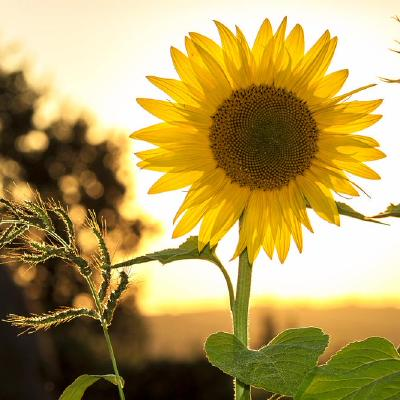
\includegraphics[width=\textwidth]{29571453.jpg}
	\caption{Figure caption here}
	\label{fig:29571453.jpg}
\end{figure}


\chapter{Summary}
\lipsum[1-5]

\addcontentsline{toc}{chapter}{Bibliography}
\bibliography{ref}{}
\bibliographystyle{unsrt}

\chapter*{List of Figures}
\addcontentsline{toc}{chapter}{List of Figures}

\chapter*{List of Tables}
\addcontentsline{toc}{chapter}{List of Tables}

\chapter*{Curriculum vitae}
\addcontentsline{toc}{chapter}{Curriculum vitae}

\noindent Personal data

\noindent\rule{\textwidth}{0.4pt}

\vskip 0.1in

\begin{tabular}{p{0.4\textwidth}p{0.6\textwidth}}
	Name: & San Zhang \\
	Date of birth: & 09.09.1999 \\
	Place of birth: & Beijing, China \\
\end{tabular} \\

\noindent Education

\noindent\rule{\textwidth}{0.4pt}

\vskip 0.1in

\begin{tabular}{p{0.4\textwidth}p{0.60\textwidth}}
	09/2018-06/2022 & Bachelor student, xxx University \\
	09/2022-06/2025 & Master student, xxx University \\
	09/2025-08/2029 & Ph.D student, xxx Berlin \\
\end{tabular} \\

\end{document}